%!TEX root = ../tesis.tex
\section{Salidas Esperadas}
\label{sec:solucion-salidas}

El resultado del algoritmo es una población final al final del periodo de estudio
de donde se puede determinar la cantidad de mosquitos hembras adultas y su posición entre otras informaciones.

La cantidad de mosquitos hembras adultas y su posición permiten evaluar el crecimiendo o decrecimiento de la población y georeferenciar los focos de la enfermedad teniendo en cuenta la densidad poblacional.

\subsection{Identificación de los focos de dengue}
Mediante los datos de entrada se podrá determinar los distintos focos de la enfermedad y su nivel de gravedad. Mediante técnicas de interpolación espacial los datos de entrada serán procesados y representados en la zona de estudio como polígonos que representan focos de la enfermedad.

\subsection{Correlación de variables}
Analizar la influencia de las variables sobre el resultado final y determinar si existen dependencias entre las mismas. Por ejemplo; analizar la influencia del par de datos de entrada (temperatura, humedad) sobre la formación de un foco de la enfermedad del dengue. Expresar la dependencia de variables, en el caso de existir, mediante un gráfico en función del tiempo para visualizar su comportamiento.

\subsection{Datos estadísticos}
Resúmenes que representan información útil dentro del marco de estudio de la enfermedad. Cantidad de infectados/habitantes de una determinada zona, Distancias entre focos más importantes de la enfermedad, lugares críticos de movimiento masivo de gente (terminal de ómnibus, centros comerciales), otros.
Cortes de tiempo e intersección de mapas
Uno de los puntos más importantes a tener en  cuenta es la evolución de los datos en función al tiempo.

\subsection{Comparación entre muestras}
Comparación entre muestras tomados de focos anteriores, para ver si hay un patrón de evolución de los focos. (Ver si se puede usar un algoritmo de detección de patrones).

\subsection{Evolución de muestras}
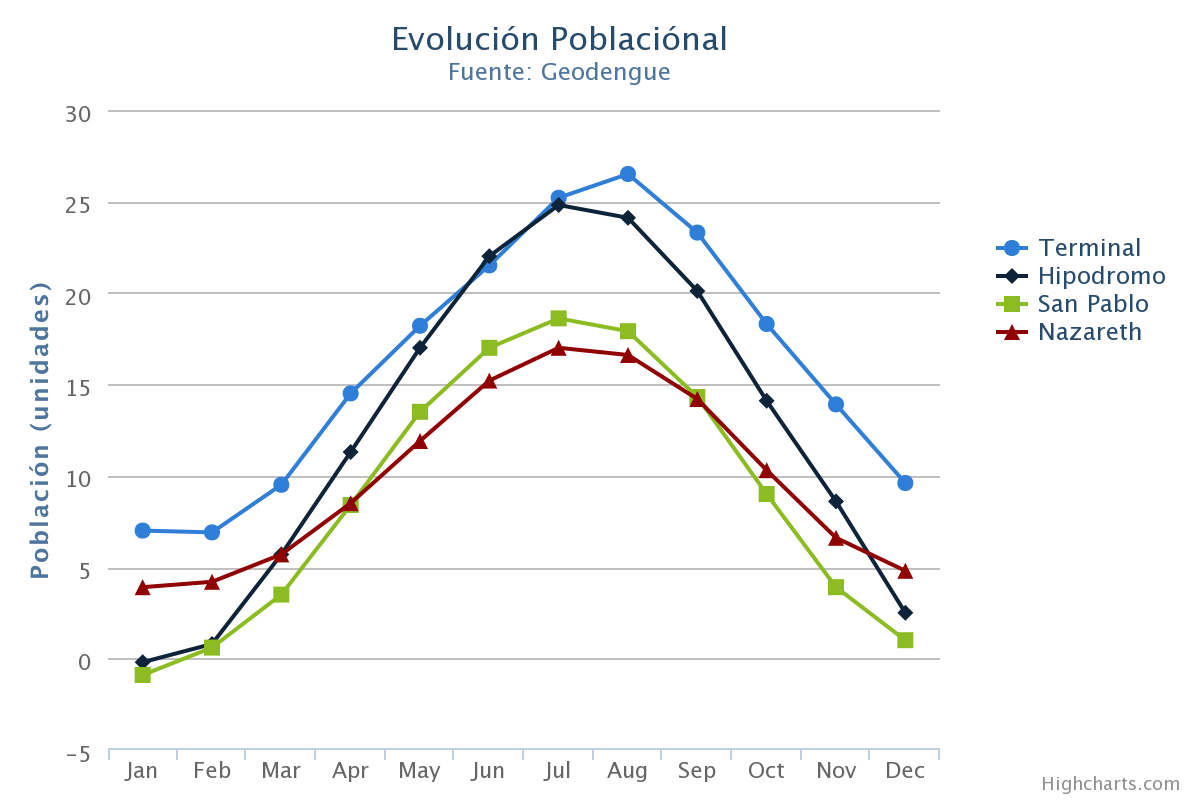
\includegraphics[ scale=0.35]{./graphics/salida-estimada.png}
El proceso de evolución de las muestras consiste en un proceso, en el cual las muestras obtenidas mediante los dispositivos de ovipostura  son expuestas a un conjunto de variaciones en un periodo de tiempo. Las variaciones que, principalmente, afectan a las muestras son
Las variaciones del clima en dicho periodo : Se someten las muestras obtenidas a las distintas variaciones climáticas ocurridas en el periodo de tiempo seleccionado para el estudio.
La naturaleza del mosquito : Cada elemento de la muestra, es sometido a cambios considerando la naturaleza del mosquito. Los aspectos que se tienen en cuenta son su ciclo de vida del mosquito, ciclo reproductivo y el desplazamiento.

\subsection{Cobertura}
*1- Comparar los layers de densidad poblacional con el de focos de dengue, el impacto que puede tener, la posible cantidad de gente a las que puede afectar el foco.
*2- Interpolar nuestras variables utilizando el método adecuado para cada variable, esto es para combinar los layers y buscarle algún significado a la combinación.
